\chapter{Stack-switching in WebAssembly}
\label{ch:appendix}

\section{Understanding Resuming and Suspending}
\label{sec:stack-switching-intuition}

A good intuition for understanding resuming and suspending in the stack-switching proposal is that it is similar to calling a function inside a try-catch block. The function can suspend by throwing different types of exceptions (suspension tags) and the try-catch block can provide different handlers for the corresponding suspension tags.

\section{WebAssembly Code Example}
\label{sec:wasm-example}

Below is a simplified example in Wasm that showcases the basics of using continuations (full example here). \texttt{\$consumer} creates a continuation object from the function \texttt{\$generator} and resumes it. When \texttt{\$generator} suspends with the tag \texttt{\$generate}, \texttt{\$consumer} jumps to the label \texttt{\$on\_generate}. At that point, the stack will contain parameters of the \texttt{\$generate} tag and a new continuation object. \texttt{\$consumer} saves the new continuation object and repeats the loop. Once \texttt{\$generator} finishes execution without suspending, \texttt{\$consumer} also returns.

\begin{lstlisting}[caption={WebAssembly stack-switching example}, label={lst:wasm-example}]
(func $generator
  ...
  (loop $loop
    ;; Suspend execution, pass current value of $i to consumer.
    (suspend $generate (local.get $i))
    ...
  )
)

(func $consumer
 ...
 ;; Create continuation executing function $generator.
 (local.set $generator_cont (cont.new $cont_type (ref.func $generator)))

 (loop $loop
   (block $on_generate (result i32 (ref $cont_type))
     ;; Resume continuation $generator_cont.
     ;; When $generate tag is thrown,
     ;; go to label $on_generate (points to right after this block)
     (resume $cont_type (on $generate $on_generate) (local.get $generator_cont))
     ;; $generator returned: no more data.
     (return)
   )
   ;; $generator suspended.
   ;; The stack now contains the value
   ;; produced by the generator and the new continuation.
   ;; Save continuation to resume it in the next iteration
   (local.set $generator_cont)
   ...
 )
)
\end{lstlisting}

\section{Control-Flow Graph}
\label{sec:control-flow-graph}

Figure~\ref{fig:stack-switching-cfg} illustrates the control flow between the \texttt{\$consumer} and \texttt{\$generator} functions, showing how stack-switching enables cooperative execution through continuations.

\begin{figure}[htbp]
\centering
\documentclass[tikz,border=10pt]{standalone}
\usepackage{tikz}
\usetikzlibrary{shapes,arrows,positioning,fit,calc}

\begin{document}
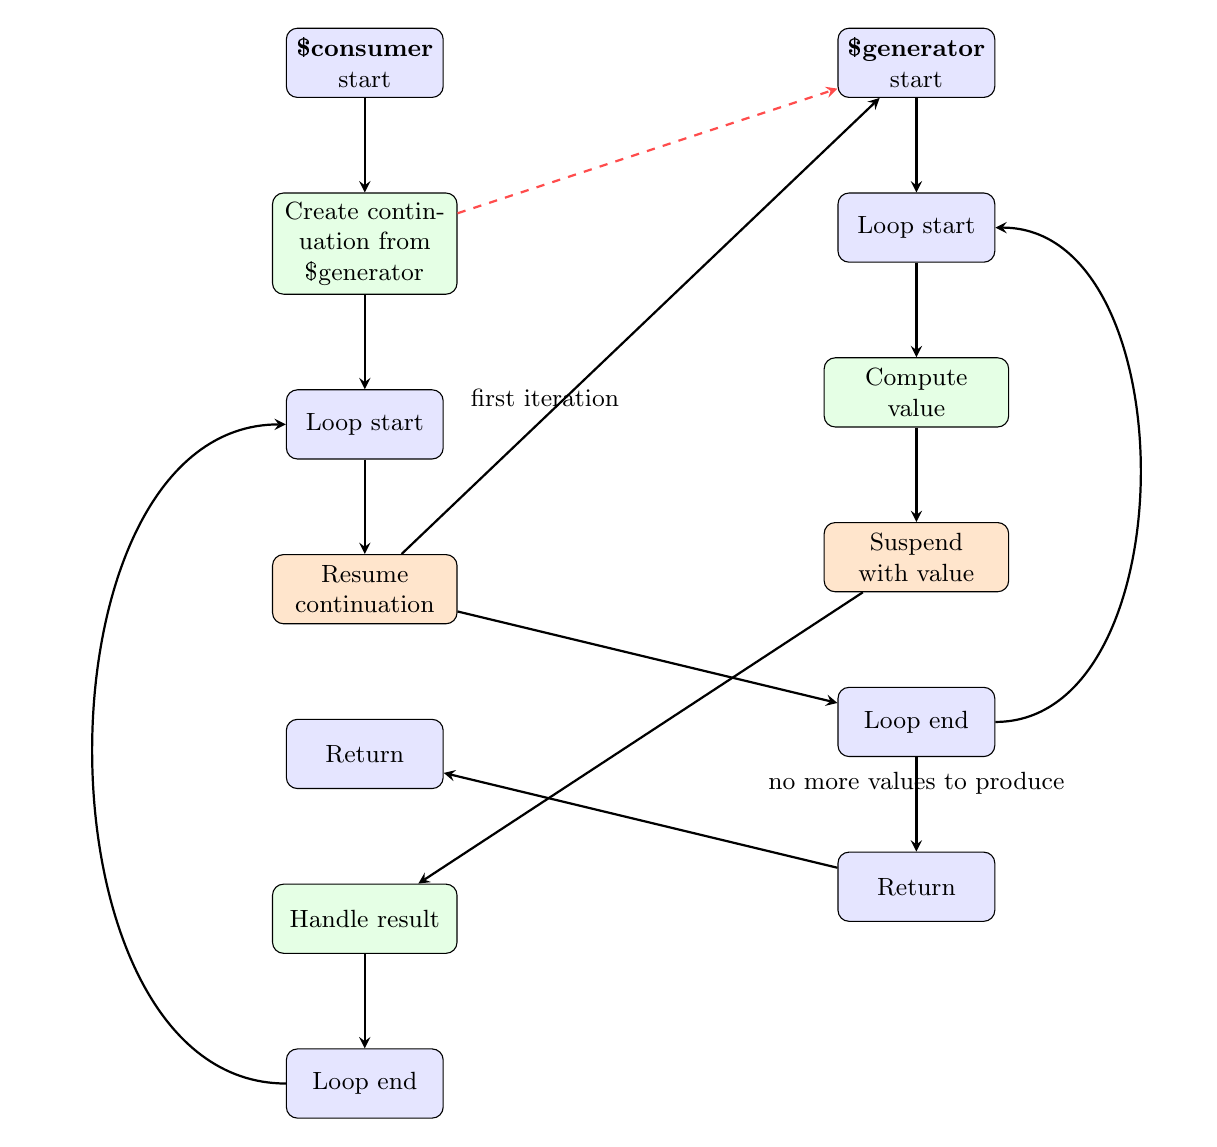
\begin{tikzpicture}[
    node distance=1.2cm and 3cm,
    every node/.style={font=\small},
    block/.style={rectangle, draw, fill=blue!10, text width=5em, text centered, rounded corners, minimum height=2.5em},
    decision/.style={diamond, draw, fill=yellow!10, text width=4em, text centered, aspect=2, inner sep=1pt},
    action/.style={rectangle, draw, fill=green!10, text width=6em, text centered, rounded corners, minimum height=2.5em},
    suspend/.style={rectangle, draw, fill=orange!20, text width=6em, text centered, rounded corners, minimum height=2.5em},
    arrow/.style={->, >=stealth, thick},
    transfer/.style={->, >=stealth, thick, dashed, color=red!70},
    solidarrow/.style={->, >=stealth, thick},
    label/.style={font=\scriptsize, text=red!70}
]

% Consumer side (left)
\node[block] (consumer-start) {\textbf{\$consumer} start};
\node[action, below=of consumer-start] (create-cont) {Create continuation from \$generator};
\node[block, below=of create-cont] (consumer-loop) {Loop start};
\node[suspend, below=of consumer-loop] (resume) {Resume continuation};
\node[block, below=of resume] (consumer-return) {Return};
\node[action, below=of consumer-return] (handle-result) {Handle result};
\node[block, below=of handle-result] (loop-end) {Loop end};

% Generator side (right)
\node[block, right=of consumer-start, xshift=2cm] (generator-start) {\textbf{\$generator} start};
\node[block, below=of generator-start] (generator-loop) {Loop start};
\node[action, below=of generator-loop] (compute) {Compute value};
\node[suspend, below=of compute] (suspend) {Suspend with value};
\node[block, below=of suspend] (loop-back-gen) {Loop end};
\node[block, below=of loop-back-gen] (generator-return) {Return};

% Consumer flow
\draw[arrow] (consumer-start) -- (create-cont);
\draw[arrow] (create-cont) -- (consumer-loop);
\draw[arrow] (consumer-loop) -- (resume);
%\draw[arrow] (resume) -- (handle-result);
\draw[arrow] (handle-result) -- (loop-end);
%\draw[arrow] (loop-end) -- (consumer-return);
\draw[arrow] (loop-end) to[out=180, in=180] (consumer-loop);

% Generator flow
\draw[arrow] (generator-start) -- (generator-loop);
\draw[arrow] (generator-loop) -- (compute);
\draw[arrow] (compute) -- (suspend);
%\draw[arrow] (suspend) -- (loop-back-gen);
\draw[arrow] (loop-back-gen) to[out=0, in=0] (generator-loop);
\draw[arrow] (loop-back-gen) -- node[above, pos=0.5] {no more values to produce} (generator-return);

% Stack-switching transfers
\draw[transfer] (create-cont) -- (generator-start);
\draw[arrow] (resume) -- node[above, pos=0.3] {first iteration} (generator-start);
\draw[arrow] (resume) -- (loop-back-gen);
\draw[arrow] (suspend) -- (handle-result);
\draw[arrow] (generator-return) -- (consumer-return);
%\draw[arrow] (handle-result) to[out=180, in=180] node[above, pos=0.5] {no value} (consumer-return);

\end{tikzpicture}

\end{document}

\caption{Control-flow graph showing stack-switching between \texttt{\$consumer} and \texttt{\$generator}. Solid arrows show sequential execution within each function. Dashed red arrows show control transfers via stack-switching operations: \texttt{cont.new} creates the continuation, \texttt{resume} transfers control to the generator, \texttt{suspend} transfers control back to the consumer with a value and updated continuation, and \texttt{return} signals completion.}
\label{fig:stack-switching-cfg}
\end{figure}
